\section{Probability, Statistics, ML, and Econometrics: Goals and Differences}


\subsection{Three Main Goals of Analyzing Data}

\begin{itemize}
    \item \textbf{Description}: Describing/Summarizing economic data
    \item \textbf{Prediction}: Predicting the future economic outcomes
    \item \textbf{Estimation of Causal Effects}: `Predicting' the differences in outcomes under various policies or interventions
\end{itemize}

\subsection{Examples of Descriptive Studies}

\subsubsection{Chetty, Hendren, Kline, and Saez (2016, QJE)}

\begin{itemize}
    \item Title: Where is the Land of Opportunity? The Geography of Intergenerational Mobility in the United States
    \item Author: Chetty, Hendren, Kline, and Saez (2016, QJE)
    \item Abstract: \textit{First, we characterize the joint distribution of parent and child income at the national level. (...) Second, intergenerational mobility varies substantially across areas within the U.S.}
    \item Data: Income data from Tax Records
    \item Question: What is the conditional distn of a child's income given their parent's income across geography?
    \item Method: Regression of the \textit{rank} of child's income on the \textit{rank} of parent's income
\end{itemize}


\subsubsection{Katz and Murphy (1992, QJE)}

\begin{itemize}
    \item Title: Changes in Relative Wages, 1963-1987: Supply and Demand Factors
    \item Author: Katz and Murphy (1992, QJE)
    \item Abstract: \textit{Movements in the college wage premium over this period appear to be strongly related to fluctuations in the rate of growth of the supply of college graduates.}
    \item Data: Wages, education, and experience from the CPS
    \item Question: How did relative wages change over time for different education/experience groups?
    \item Method: Comparisons of the \textit{quantiles} of earnings over time by education/experience groups
\end{itemize}

\subsection{Examples of Prediction Studies}

\subsubsection{Campbell Harvey (1989, Financial Analysts Journal)}

\begin{itemize}
    \item Title: Forecasts of Economic Growth from the Bond and Stock Markets
    \item Author: Campbell Harvey (1989, Financial Analysts Journal)
    \item Data:  Quarterly growth in real GDP, yield spread between long- and short-run annualized yields, S\&P 500
    \item Question: What predicts growth rate? Does the yield spread do better than the stock market in predicting GDP growth? (a purely forecasting problem)
    \item Method: Linear Regression
\end{itemize}

\subsubsection{Predicting Handwritten Digits(MNIST)}

\begin{itemize}
    \item Data: $Y_i \in \{0, 1, 2, ..., 9\}$ is the digit label, $X_i \in \mathbb{R}^{784}$ is the pixel information(black/white) for 400 pixels
    \item Question: What is the most likely outcome for $Y_i$ given $X_i=x$?
    \item Method: A bunch
\end{itemize}

We wouldn't need or want confidence intervals for this problem, since we are only interested in the most likely outcome and the accuracy of the prediction.

\subsubsection{Netflix Challenge}

\begin{itemize}
    \item Data: Characteristics of the movies and the characteristics of the users(including past rental behavior)
    \item Goal: Recommend movie given the characteristics of the user and the movie
\end{itemize}

\subsection{Examples of Causal Studies}

\subsubsection{Card and Krueger (1996, AER)}

\begin{itemize}
    \item Title: Minimum Wages and Employment: A Case Study of the Fast Food Industry in New Jersey and Pennsylvania
    \item Author: Card and Krueger (1996, AER)
    \item Abstract: \textit{Comparisons of employment growth at stores in New Jersey and Pennsylvania (where the minimum wage was constant) provide simple estimates of the effect of the higher minimum wage.}
    \item Data: Employment data from Fast Food Restaurants in NJ and PA in early and late 1992
    \item Question: What is the \textit{causal} effect of a minimum wage increase on employment in NJ?
    \item Method: Difference-in-differences regression
\end{itemize}


\subsubsection{Imbens, Rubin, and Sacerdote (2001, AER)}

\begin{itemize}
    \item Title: Estimating the Effect of Unearned Income\footnote{The unearned income here is the social security earnings from individuals who played and won the lottery, which is a guaranteed income for an almost lifelong period.} on Labor Earnings, Savings, and Consumption: Evidence from a Survey of Lottery Players
    \item Author: Imbens, Rubin, and Sacerdote (2001, AER)
    \item Abstract: \textit{This paper provides empirical evidence about the effect of unearned income on earnings, consumption, and savings.}\footnote{Guido: The original motivation of this paper was to estimate the impact of poverty on children's future income.}
    \item Data: Social security earnings from individuals who played and won the lottery.
    \item Question: What is the \textit{causal} effect of lottery winnings on labor earnings?
    \item Method: Linear Regression
\end{itemize}


The lottery participants might have different characteristics from the non-lottery participants, which raises a question regarding \textbf{external validity}.
To address this, the paper compares the individuals from the lottery data to CPS and looked at the income distribution. Here, the authors found that the distribution of earnings is similar to that of the CPS.

\subsubsection{Aviv Nevo (2001, Econometrica)}

\begin{itemize}
    \item Title: Measuring Market Power in the Ready-to-Eat Cereal Industry
    \item Author: Aviv Nevo (2001, Econometrica)
    \item Abstract: \textit{I estimate price-cost margins, but more importantly I am able empirically to separate these margins into three sources}
    \item Data: Quantities and prices of cereals for different brands, in different cities, over time.
    \item Question:  Is this industry a classic example of a concentrated differentiated products industry in which price competition is approximately cooperative and rivalry is channeled into advertising and new product introduction?
    \item Method: \textit{Structural Model} of Supply and Demand
\end{itemize}


\subsection{Probability and Statistics}


\begin{itemize}
    \item Probability: Given a \textbf{fully specified\footnote{Probability model is fully specified if it specifies the probability of every event in the sample space. (which implies having all the parameters and the functional form of the model known)}} probability model, what are the probabilities of particular events / the probability of particular events conditional on other events?
    \item Statistics: Given the \textbf{realizations} of a random variable $Y$, drawn from a distribution $F_\theta$, what can we say about the parameters $\theta$?
    \begin{itemize}
        \item $Y$ may be a vector of observations and $\theta$ may be a finite dimensional vector or an unkown function.
        \item \textbf{Estimation}: What is a good estimate of $\theta$ given the realization of $Y$?
        \item \textbf{Testing}: Is $\theta = \theta_0$ consistent with the observation $Y$?
    \end{itemize}
\end{itemize}

\subsubsection{Estimation}

Suppose we have a random sample $Y_1, \ldots, Y_N$ drawn from a distribution $N(\theta, 1)$, and we want to estimate the parameter $\theta$.
What is a good estimate of $\theta$? The most natural estimator is the sample mean $\hat{\theta} = \frac{1}{N}\sum_{i=1}^N Y_i$, which is both the \textbf{maximum likelihood estimator} and the \textbf{least squares estimator}.
In this case, $\hat{\theta}$ has the following properties:

\begin{itemize}
    \item \textbf{Normality}: $\hat{\theta} \sim N(\theta, \frac{1}{N})$
    \item \textbf{Unbiasedness}: $\E(\hat{\theta}) = \theta$
    \item \textbf{Efficiency}: $\hat{\theta}$ is the most efficient estimator of $\theta$ among all unbiased estimators (we can't do any better than this)\footnote{NB: It touches the Cramér-Rao lower bound. This is a direct case of the Rao-Blackwell Theorem.q1s2}
\end{itemize}

\subsubsection{Testing}

Why and when are we interested in testing?

\begin{itemize}
    \item In the medical/physics settings, $\theta\neq\theta_0$ itself might be interesting.
    \item In the social science settings, we want to see the ``magnitude'' of the results, and whether we have enough evidence for a certain claim.
    \item In many of theses cases, we don't want to switch to a different model arbitrarily.
    \item However, the general rule of $|t| > 2$ is completely arbitrary. In terms of decision-making, relying on tests is not a good idea.
\end{itemize}

\subsection{Machine Learning}

\subsubsection{Linear Regression}
Suppose we have a predictive linear model with large number of parameters $K$:

$$
Y_i = \beta_0 + \beta_1 X_{i1} + \beta_2 X_{i2} + \cdots + \beta_K X_{iK} + \varepsilon_i
$$

where $X_{i1}, X_{i2}, \ldots, X_{iK}$ are the features and $\beta_0, \beta_1, \ldots, \beta_K$ are the parameters.
Then, $\hat{Y}_{N+1}$ is not a very good estimator for either $Y_{N+1}$ or $\E(Y_{N+1}|X_{N+1})$.

The typical solution is to \textbf{regularize} the estimator. For example,

\begin{align}
    \min_\beta = \sum_{i=1}^N (Y_i - \beta_0 - \beta_1 X_{i1} - \beta_2 X_{i2} - \cdots - \beta_K X_{iK})^2 + \lambda \sum_{j=1}^K |\beta_j|
\end{align}

is the \textbf{lasso} estimator, which \textit{shrinks} the coefficients towards zero. This leads to a better out-of-sample performance.

Going a little further, the LASSO regularization parameter $\lambda$ is often chosen using cross-validation. For example, we can consider the \textbf{leave-one-out cross-validation (LOOCV)}:

Define 

\begin{align}
    \beta^{(i)}(\lambda) = \arg\min_{\beta} \sum_{j\neq i} (Y_j - \beta_0 - \beta_1 X_{j1} - \beta_2 X_{j2} - \cdots - \beta_K X_{jK})^2 + \lambda \sum_{k=1}^K |\beta_k|
\end{align}

based on least squares omitting the $i$-th observation. Then, the LOOCV error is given by:

\begin{align}
    Q(\lambda) = \frac{1}{N} \sum_{i=1}^N (Y_i - \hat{\beta}^{(i)}(\lambda)_0 - \hat{\beta}^{(i)}(\lambda)_1 X_{i1} - \hat{\beta}^{(i)}(\lambda)_2 X_{i2} - \cdots - \hat{\beta}^{(i)}(\lambda)_K X_{iK})^2
\end{align}

From this, we can choose the $\lambda$ that minimizes the LOOCV error: $\hat{\lambda} = \arg\min_\lambda Q(\lambda)$.

\subsubsection{Kernel Methods}

Another thing that can be done is using nonparametric models($\E[Y_i|X_i=x] = g(x)$). If $X_i$ is low-dimensional, traditional researchers use \textbf{kernel} methods:

\begin{align}
    \hat{g}(x) = \sum_{i=1}^N K(\frac{X_i - x}{h}) Y_i \Big/ \sum_{i=1}^N K(\frac{X_i - x}{h})
\end{align}

\subsubsection{Neural Nets}

However, Kernel methods do not work well if $X_i$ is high-dimensional.
In this case, \textbf{deep neural networks} are often used.

\begin{align}
    g(x) = \gamma_0 + \sum_{s=1}^S \gamma_s h\biggl(\sum_{j=1}^J \beta_{sj} x_j\biggr)\label{eq:neural_net}
\end{align}

Equation \ref{eq:neural_net} is an example of a \textbf{two-layer neural network}, where the \textit{activation function} $h(\cdot)$ is fixed and we estimate $S\times J$ parameters $\beta_{sj}$ and $S+1$ parameters $\gamma_s$.
The \textbf{ReLU} function is a popular activation function($h(z) = \max(0, z)$) to introduce non-linearity.

\subsection{What is Econometrics?}

Econometrics is not solely about predictions, but also (primarily) about causal effects:

\begin{itemize}
    \item What is the causal effect of raising the minimum wage on employment?
    \item What is the causal effect of getting more education on earnings?
\end{itemize}

These questions require dealing with \textbf{endogeneity, exogeneity, and identification}.
For example, people who \textit{choose} to get more education may do so precisely because they are more likely to be high-ability individuals, and their expected returns to education are higher.

\subsubsection{Ed Leamer(1983, AER)}

\begin{quote}
    ``The applied econometrician is like a farmer who notices that the yield is
    somewhat higher under trees where birds roost, and he uses this as evidence
    that bird droppings increase yields. However, when he presents this finding at
    the annual meeting of the American Ecological Association, another farmer
    in the audience objects that he used the same data but came up with the
    conclusion that moderate amounts of shade increase yields. A bright chap in
    the back of the room then observes that these two hypotheses are indistin-
    guishable, given the available data. He mentions the phrase "identification
    problem," which, though no one knows quite what he means, is said with
    such authority that it is totally convincing.''
\end{quote}

Bottom Line: What makes econometrics different from other data analysis is that we are interested in identification. There are settings where we have a clear definition of ``identification'', a lot of cases we don't.


\subsubsection{Classical Econometric Example: Supply and Demand}

In the supply and demand model, we know that the prices are not set \textit{randomly} but deliberately in response to demand.
We cannot estimate a demand function by simply comparing sales when prices are high and when prices are low. Instead, we build a \textit{model} for the behavior of buyers and sellers:

\begin{align}
    Q_d(P) &= \alpha_0 + \alpha_1 P + \alpha_2 Y + \varepsilon_d \label{eq:demand_function}\\
    Q_s(P) &= \beta_0 + \beta_1 P + \beta_2 W + \eta_s \label{eq:supply_function}
\end{align}

We consider the following equation of the \textbf{equilibrium condition}:

\begin{align*}
    Q_d(P) = Q_s(P)
\end{align*}


\newpage

\section{Randomization and Fisher's Exact P-Values}
\label{sec:randomization_and_fisher_s_exact_p_values}

\subsection{Introduction to Causal Inference}

There are three key notions underlying the general approach to causality:

\begin{enumerate}
    \item \textbf{Potential Outcomes}: Each outcome corresponding to the various levels of a treatment or manipulation
    \item \textbf{Multiple Units and Stability(SUTVA)}
    \item \textbf{\color{red}Assignment Mechanism}: Why some are exposed to the treatment and some are not(crucial for inferring causal effects and serves as an organizing principle)
\end{enumerate}


\subsection{The Fundamental Problem of Causal Inference}

Suppowe we have a binary outcome/manipulation/treatment/cause variable $W_i \in \{0, 1\}$ for all $i=1, \ldots, N$.

We associate each action with a potential outcome:
\begin{itemize}
    \item $Y_i(0)$: The outcome for the $i$-th unit if they are \textit{not} exposed to the treatment
    \item $Y_i(1)$: The outcome for the $i$-th unit if they are exposed to the treatment
\end{itemize}

We would want to compute the \textbf{unit-level causal effects}(i.e., the direct comparison of the two potential outcomes) for each unit.
For example, $\tau_i:= Y_i(1) - Y_i(0)$ or $\tau_i:= Y_i(1) / Y_i(0)$.

However, we observe only one value of $W_i$, and therefore only one of the potential outcomes is ever observed:

\begin{align}
Y^{obs} \equiv Y(W) &= \begin{cases}
    Y_i(0) & \text{if } W_i = 0 \\
    Y_i(1) & \text{if } W_i = 1
\end{cases}\\
Y^{mis} \equiv Y(1-W) &= \begin{cases}
    Y_i(1) & \text{if } W_i = 0 \\
    Y_i(0) & \text{if } W_i = 1
\end{cases}
\end{align}

Such situation, the fact that it is impossible to observe all components of the causal effects($\tau_i$) is called the \textbf{fundamental problem of causal inference}.


\subsection{Why potential outcomes are useful}

Potential outcome notion is consistent with the way economists traditionally think about demand/supply or production functions:

\begin{align*}
    q^d(p)\text{ and } q^s(p)
\end{align*}

Some causal questions are more challenging, including estimating the causal effect of ``immutable'' characteristics on economic outcomes. One solution is to make manipulation precise.
For example, \textcite{bertrand2004emily} do not manipulate the ethinicty itself, but they manipulate the ``perceived'' ethnicity of the applicants.
In such case and most causal questions, we must be exact about what the manipulation is.
We would have to ask the following questions:

\begin{itemize}
    \item Can we see causal effects here?
    \item Can we do experiments in this case?
    \item What's the treatment here?
\end{itemize}


\subsection{Leveraging Multiple Units}

Because we cannot learn much about causal effects from a single observed outcome, we typically rely on multiple units to learn about causal effects.
This does not come without any assumptions. In some cases, one's potential outcomes may be \textit{dependent} on the potential outcomes of others.
For example, in agricultural fertilizer experiments, researchers have taken care to separate plots using ``guard rows'', or unfertilized strips of land between fertilized areas.
In other words, if we have \textbf{spillovers}, changing the treatment for one unit may affect the potential outcomes of other units; such spillover effects are the main focus in the peer effects / social interactions litearture,
but in most of our discussion, we will assume that the potential outcomes are independent of each other. i.e., We make the \textbf{Stable Unit Treatment Value Assumption (SUTVA)}:

\begin{align*}
    Y_i(1), Y_i(0) \text{ are independent of } Y_j(1), Y_j(0) \text{ for all } i \neq j
\end{align*}

This assumption is crucial for the identification of causal effects.

\subsection{Assignment Mechanism}

A key ingredient is how each individual came to receive the treatment level:

\begin{align}
    Pr(W|Y(1), Y(0), X)
\end{align}

We can partition the cases into the following three categories:

\begin{itemize}
    \item \textbf{Random Assignment}: known, no dependence on $Y(1), Y(0)$
    \item \textbf{Unconfounded Assignment, Stratified Random Design}: unknown, no dependence on $Y(1), Y(0)$
    \item \textbf{Confounded Assignment}: unknown, possible dependence on $Y(1), Y(0)$ $\rightarrow$ the most challenging case
\end{itemize}

In the case of random assignment, we can use the potential outcomes to identify the causal effects.
In the case of non-random assignment, we need to make some assumptions to identify the causal effects.

\clearpage

\subsection{Random Assignment}

\begin{itemize}
    \item Finite population with $N$ units
    \item $M$ units are selected at random to receive the treatment; the remaining $N-M$ units receive the control
    \item The assignment probability is given by:
    \begin{align}
        Pr(\mathbf{W} = \mathbf{w}) = \binom{N}{M}^{-1}
    \end{align}
    \item There are $\binom{N}{M}$ possible assignment vectors $\mathbf{w}$, \textbf{all equally likely}
    \item Special case of equal size treatment and control groups: $M = N/2$
\end{itemize}

\subsubsection*{cf) Bernoulli Trials}

A slightly different setting from the one above is the \textbf{Bernoulli trials} with 

\begin{align}
    Pr(W = w) = 2^{-N} \quad \forall w \in \{0, 1\}^N
\end{align}

This is a slightly \textit{less attractive} setting than below – we might end up with highly imbalanced treatment and control groups, and in the worst case, we might not be able to identify the causal effects by ending up with a single treatment or control group.


\subsection{Exact Tests}

Moving away from the course material, let's first review the basics of hypothesis testing.

A test is a function of the data that maps the data to a decision to reject or not reject the null hypothesis.
The term \textbf{exact test} refers to a hypothesis test whose \textbf{p-value} is exactly computable from the distribution of the test statistic under the null hypothesis.
\textit{This is different from the \textbf{asymptotic(large-sample) approximation} such as the normal, t, or chi-squared distribution.}
We say that the p-value\footnote{Def: The sum of the probabilities of equi-likely or less likely events under the null hypothesis.} is \textbf{exact} in the sense that it is derived directly from the true null distribution. Formally,

\begin{align}
    p = \sum_{x\in \mathcal{X}} P_{H_0}(X=x)
\end{align} 

where $\mathcal{X}$ is the set of all possible ``extreme'' cases of the data under the null hypothesis.


{\color{blue}

TBU: Can assuming the error term being exactly normally distributed and then running t-test on the regression coefficients be considered as an exact test?
}


\subsection{Sharp Null Hypothesis}

Given data from a completely randomized experiment, Fisher (1935) was interested in testing \textbf{sharp null hypotheses}—that is, null hypotheses under
which all values of the potential outcomes for the units in the experiment are either observed or can be specified.
This is distinct from the null hypothesis that the average treatment effect is zero, which is not a sharp null hypothesis.
The null of a zero average is a weaker hypothesis because the average effect of the treatment may be zero even if for some units the treatment has a positive effect, as long as for others the effect is negative.

For example, a \textbf{sharp null hypothesis} can be written as:

\begin{align*}
    H_0&: Y_i(1) = b_i\cdot Y_i(0) + c_i \quad \forall i\\
    H_1&: Y_i(1) \neq b_i\cdot Y_i(0) + c_i \quad \text{for some } i
\end{align*}

For now, let us focus on the hypothesis $H_0: Y_i(1) = Y_i(0) \quad \forall i$. When is this sharp null with zero individual treatment effects more interesting than the null of a zero average treatment effect? If the change in outcome of any individual is important itself, then the sharp null is more interesting.
However, if we want to know the overall direction of the treatment effect, then the null of a zero average treatment effect is more interesting.

\subsection{Test Statistic}

From now on, we will assume that the total number of units in our finite population is $N$< and the total number of units that receive the treatment is fixed at$M$:

\begin{align}
    M = \sum_{i=1}^N W_i
\end{align}

In this \textbf{fixed $M$ design}, we have

\begin{align}
    Pr_\text{fixed}(\mathbf{W} &= \mathbf{w}) = Pr_\text{fixed}(\mathbf{W} = \mathbf{w}| M) Pr_\text{fixed}(M)\\
    &= Pr_\text{fixed}(\mathbf{W} = \mathbf{w}| M) = \binom{N}{M}^{-1}
\end{align}

A \textbf{test statistic} is a known function $T=T(\mathbf{W}; Y^{obs}, X)$ of the assignment vector $\mathbf{W}$, observed outcomes $Y^{obs}$, and \textit{pretreatment} covariates $X$.

The stochasticity of $T$ is solely due to the stochastic nature of the assignment vector $\mathbf{W}$, leading to the \textbf{randomization distribution}\footnote{i.e., the histogram of all values for the statistic from all possible ways the experimental units could have been randomly assigned to the treatment and control groups.} of $T$.

sing this distribution, we can compare the observed test statistic $T^{obs}$ agains its distribution under the null hypothesis to compute the p-value.

\vspace{1em}

Question: What are the two ingredients for Fisher's exact test approach?

{\color{gray}
\begin{itemize}
    \item The choice of the null hypothesis
    \item The choice of the test statistic
\end{itemize}
}


\subsubsection{The Rank Statistic}

An important class of statistics involves transforming the outcomes to \textbf{rank} statistics before considering the differences by treatment status.
This improves robustness (against skewness and outliers) relative to difference-in-means without having to make an arbitrary choice such as taking logs; however, it must be noted that it is not a good idea to use it with data that is zero-inflated.

In practice, we also subtract $(N+1)/2$ from each to obtain a \textbf{normalized rank} statistic that has average zero in the population:

\begin{align}
    R_i(Y_1^{obs}, Y_2^{obs}, \dots, Y_N^{obs}) &= \sum_{j=1}^N \mathbf{1}\{Y_j^{obs} < Y_i^{obs}\} + \frac{1}{2}\biggl(1+\sum_{j=1}^N \mathbf{1}\{Y_j^{obs} = Y_i^{obs}\}\biggr) - \frac{N+1}{2}
\end{align}

Given the ranks $R_i$, an attractive test statistic is the difference in average ranks for the treated and control units:

\begin{align}
T = \frac{\sum_i W_iR_i}{\sum_iW_i} - \frac{\sum_i (1-W_i)R_i}{\sum_i (1-W_i)}
\end{align}

This statistic is invariant to monotone transformations of the outcomes and is zero under the sharp null.

\subsection{Exact Test Procedure}

\begin{enumerate}
    \item Specify the null hypothesis $H_0$
    \begin{align}
        H_0: Y_i(1) = Y_i(0) \quad \forall i
    \end{align}
    \item Choose the test statistic $T$
    \begin{itemize}
        \item \textbf{Difference-in-means}: $T = \frac{1}{N}\sum_{i=1}^N (W_iY_i - (1-W_i)Y_i)$
        \item \textbf{Difference-in-medians}: $T = \text{median}(W_iY_i) - \text{median}((1-W_i)Y_i)$
        \begin{itemize}
            \item[:]robust against outliers, but not against zero-inflated data
        \end{itemize}
        \item \textbf{Difference in average normalized ranks}: $T = \frac{1}{N}\sum_{i=1}^N \frac{rank(W_iY_i) - rank((1-W_i)Y_i)}{N}$
        \begin{itemize}
            \item[:]robust agianst outliers, but not against zero-inflated data(though better than the difference-in-medians)
        \end{itemize}
    \end{itemize}
    \item Compute the observed test statistic $T^{obs}$
    \item Compute $T$ for all other possible assignment vectors $\mathbf{w}$(depends on the \textbf{randomization scheme})
    \begin{itemize}
        \item If the population size $N$ is large, it is computationally difficult to compute all possible assignment vectors $\mathbf{w}$
        \item Instead, we can consider a large enough number of permutations of the treatment assignment to approximate the randomization distribution.(Details in section \ref{sec:computation_of_p_values_with_large_n})
    \end{itemize}
    \item Compute the p-value as the sum of the probabilities of all values of $T$ that are as or more extreme than the observed test statistic $T^{obs}$
\end{enumerate}

\subsubsection{Computation of P-values with large $N$}
\label{sec:computation_of_p_values_with_large_n}

The p-value calculations so far have been exact.
With large $N$, it may be infeasible to calculate the test statistic for every value of the assignment vector.
In this case we rely on \textit{numerical approximations} to compute the p-value.
Formally, we randomly draw $N$-dimensional vector with $N-M$ zeros and $M$ ones from the set of assignment vectors $K$ times.
We then approximate the p-value for our test statistic by the fraction of these $K$ statistics that are at least as extreme in absolute values as $|T^{obs}|$.


\begin{algorithm}
    \caption{Exact Test Procedure (with numerical approximation)}
    \label{alg:exact_test_procedure}
    \begin{algorithmic}
        \State Given $N, M, Y^{obs}, T(\cdot)$
        \State Initialize $T^{sim}$
        \State $T^{obs} \gets T(W, Y^{obs})$
        \State $K \gets 100000$
        \For{$k \in 1, \ldots, K$}
        \State $\mathbf{w}_k \gets \text{random permutation of } \{0, 1\}^N$
        \State $T^{sim}_k \gets T(\mathbf{w}_k, Y^{obs})$
        \State $T^{sim} \gets T(\mathbf{w}, Y^{obs}, X)$
        \EndFor
        \State Return $p$-value = $\frac{1}{K} \sum_{k=1}^K \mathbf{1}\{|T^{sim}_k| \geq |T^{obs}|\}$
    \end{algorithmic}
\end{algorithm}


\newpage

\subsection*{W. The thought that larger $|T|$ are more unlikely, is this an assumption or a fact?}

\begin{figure}[ht]
    \centering
    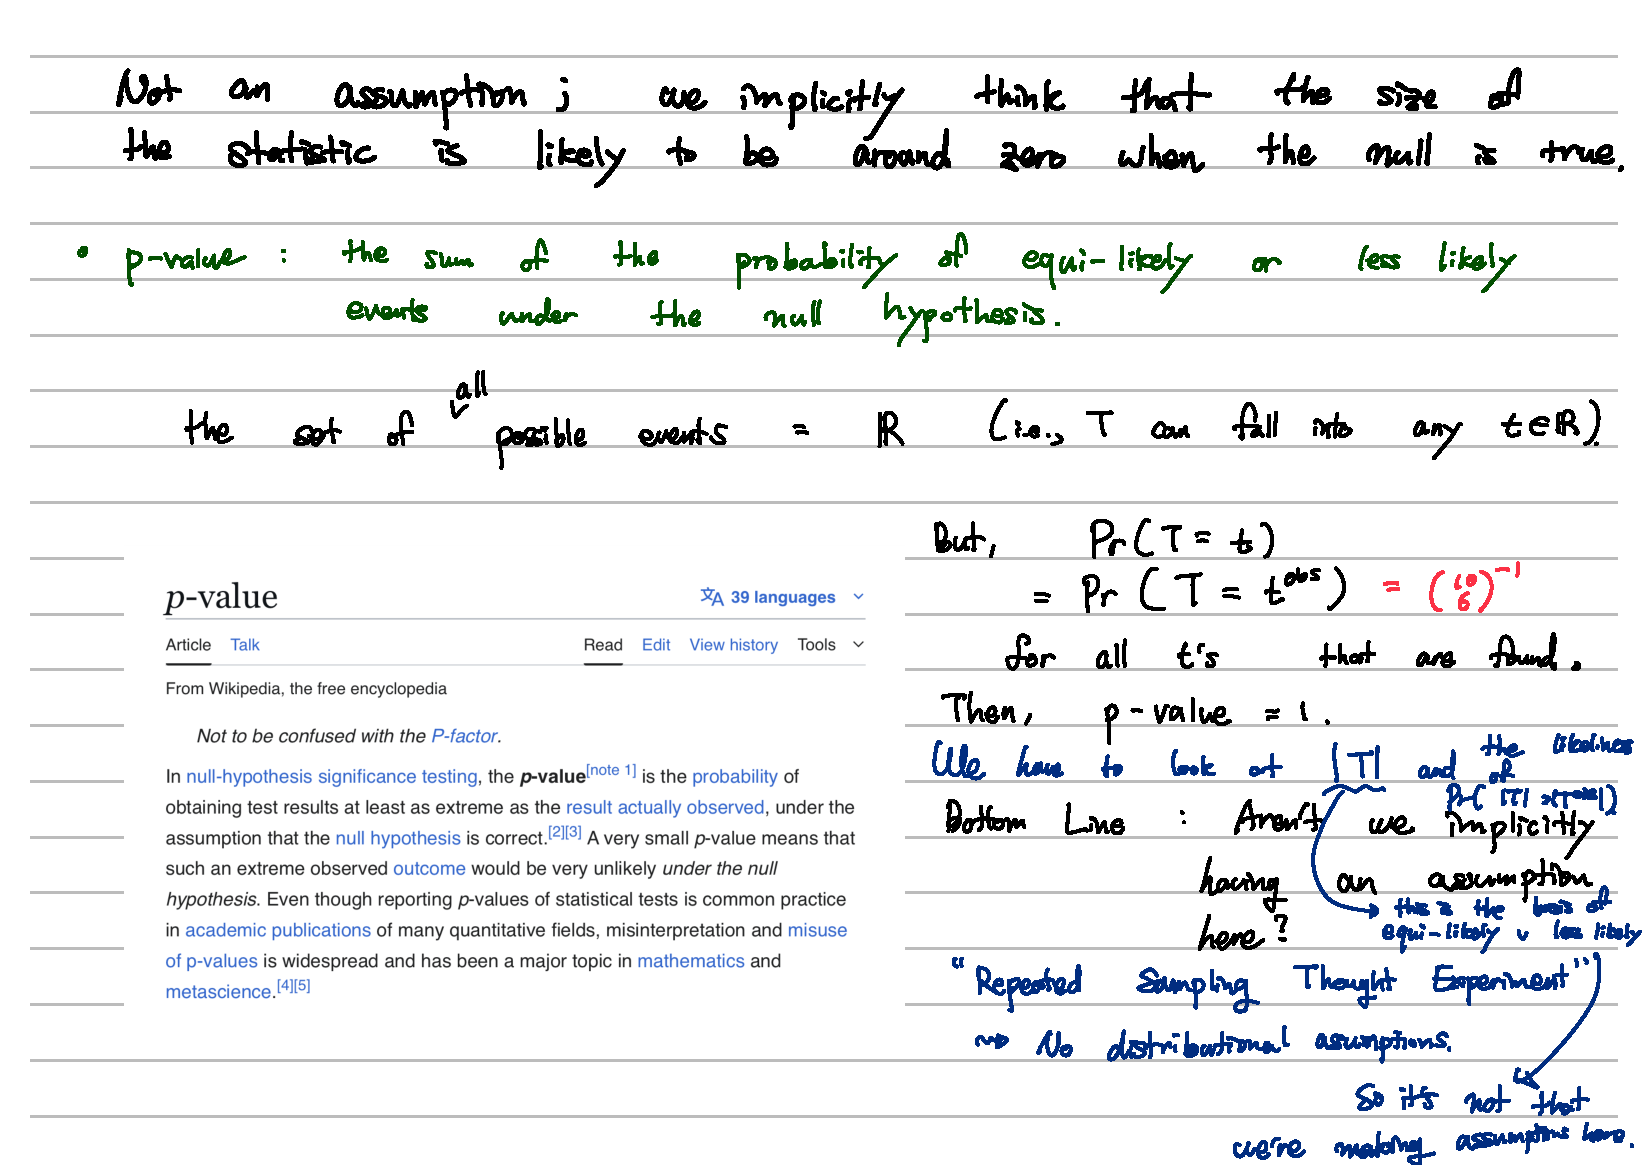
\includegraphics[width=\textwidth]{figures/sec2-1.pdf}
\end{figure}

\newpage

\subsection{Takeaways}

\begin{itemize}
    \item {\color{blue} Testing based on random sample is different from testing for the population. There is no approximation or further assumptions in this case, and the source of randomness is not from the random sampling scheme. It is only the randomization itself that helps us understand the data.}    
    \item Randomization-based p-values underlie tests for treatment effects.
    \item In practice, using approximations to p-values based on normal approximations to the distribution of the t-statistic is often similar to the exact p-values to the exact p-vlaues based on difference-in-means test.
    \begin{itemize}
        \item[$\because$] The t-statistic should be normally distributed in large samples by CLT.
    \end{itemize}
    \item With very skewed distributions rank-based tests are much better, but one needs to be careful regarding the presense of masspoints.
\end{itemize}